% Copyright (C) 2012 Shi.Zhan <g.shizhan.g@gmail.com>
%
% Permission is hereby granted, free of charge, to any person obtaining a copy of this software and associated documentation files (the "Software"), to deal in the Software without restriction, including without limitation the rights to use, copy, modify, merge, publish, distribute, sublicense, and/or sell copies of the Software, and to permit persons to whom the Software is furnished to do so, subject to the following conditions:
%
% The above copyright notice and this permission notice shall be included in all copies or substantial portions of the Software.
%
% THE SOFTWARE IS PROVIDED "AS IS", WITHOUT WARRANTY OF ANY KIND, EXPRESS OR IMPLIED, INCLUDING BUT NOT LIMITED TO THE WARRANTIES OF MERCHANTABILITY, FITNESS FOR A PARTICULAR PURPOSE AND NONINFRINGEMENT. IN NO EVENT SHALL THE AUTHORS OR COPYRIGHT HOLDERS BE LIABLE FOR ANY CLAIM, DAMAGES OR OTHER LIABILITY, WHETHER IN AN ACTION OF CONTRACT, TORT OR OTHERWISE, ARISING FROM, OUT OF OR IN CONNECTION WITH THE SOFTWARE OR THE USE OR OTHER DEALINGS IN THE SOFTWARE.
%
% 课程:人机交互技术及应用
% 班级:传播学1001班
% 课时:40学时,2012年秋季1~10周,每周一、三
% 地点:东九楼D212
% 主页:http://code.google.com/p/hci-course/
% 教师:施展
% 单位:华中科技大学 武汉光电国家实验室
%
\documentclass{beamer}
\usepackage{fontspec,xunicode,xltxtra,beamerthemesplit}
%\usetheme{Hannover} % White background
\usetheme{Berkeley} % Blue background
\setsansfont[Mapping=tex-text, ItalicFont={Courier Italic}]{Microsoft YaHei}

% 中文环境自动换行
\XeTeXlinebreaklocale "zh"
\XeTeXlinebreakskip = 0pt plus 1pt

% 中文环境修正导航栏
\makeatletter
\def\beamer@linkspace#1{%
  \begin{pgfpicture}{0pt}{-1.5pt}{#1}{5.5pt}
    \pgfsetfillopacity{0}
    \pgftext[x=0pt,y=-1.5pt]{.}
    \pgftext[x=#1,y=5.5pt]{.}
  \end{pgfpicture}}
\makeatother

% diagrams
\usepackage{tikz}
\usetikzlibrary{arrows,positioning} 
\tikzset{
    %Define standard arrow tip
    >=stealth',
    %Define style for boxes
    punkt/.style={
		rectangle,
		rounded corners,
		draw=black, very thick,
		text width=6.5em,
		minimum height=2em,
		text centered},
	line/.style = {
		->,
		draw,
		text centered,
		-latex'}
}

\title{人机交互技术}
\author{施展}
\institute{华中科技大学~武汉光电国家实验室}
\date{{\small \today}}
\titlegraphic{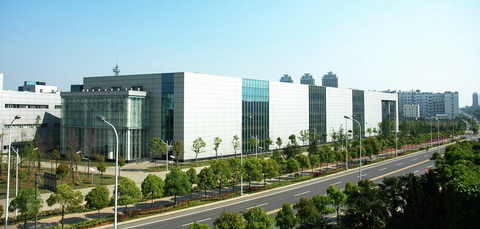
\includegraphics[width=3.5cm]{images/wnlo.jpg}}

\begin{document}

\begin{frame}
	\titlepage
\end{frame}

\begin{frame}
 	\tableofcontents
\end{frame}

\section{课程介绍}
\subsection{教材及参考书}
\begin{frame}
	\frametitle{教材及参考书}
    \transdissolve
	\begin{columns}
		\column{5cm}
			\centerline{\includegraphics[width=2.7cm]<1->{images/textbook.jpg}}\label{textbook}
		\column{5cm}
			\centerline{\includegraphics[width=2.7cm]<2->{images/referencebook.jpg}}\label{referencebook}
	\end{columns}
    \beamertemplatetransparentcovereddynamicmedium
	\begin{itemize}
		\item<1->[教材] {\tiny 孟祥旭,李学庆,杨承磊等:《人机交互基础教程(第2版)》清华大学出版社,2010}
		\item<2->[参考] {\tiny [美]施奈德曼,[美]普莱萨特,《用户界面设计—有效的人机交互策略(第五版)》,2010}
	\end{itemize}
\end{frame}

\subsection{教学目标}
\begin{frame}
	\frametitle{教学目标}
	\beamertemplatetransparentcovereddynamicmedium 
	\begin{itemize}[<+-|alert@+>]
		\item 了解人机交互的含义~{\tiny 人机交互的研究内容及发展趋势}
		\item 了解人机交互的一些新技术~{\tiny 语音、手写识别、眼动跟踪等技术}
		\item 掌握人机交互的表示模型~{\tiny 能够进行形式化的描述}
		\item 掌握人机交互界面构造的一般性方法~{\tiny 能着手设计人机交互界面程序}
		\item 掌握认知心理学、人机工程学在人机界面的作用~{\tiny 能够初步运用相关知识进行人机交互界面评价}
		\item 了解Web界面和移动界面设计的发展趋势~{\tiny 初步认识Web界面和移动界面设计时需注意的特殊问题}
	\end{itemize}
\end{frame}

\subsection{教学内容}
\begin{frame}
	\frametitle{教学内容}
	\beamertemplatetransparentcovereddynamicmedium
	\begin{itemize}[<+-|alert@+>]
		\item 人机交互概念
		\item 感知和认知基础
		\item 交互设备
		\item 交互技术
		\item 界面设计 
		\item 人机交互的界面表示模型与实现
		\item Web界面设计
		\item 移动界面设计
		\item 可用性分析与评估
	\end{itemize}
\end{frame}

\subsection{联系方式}
\begin{frame}
	\frametitle{联系方式}
	\beamertemplatetransparentcovereddynamicmedium
	\transwipe
	\begin{center}
		\includegraphics[scale=.5]<1>{images/maps.google.com_2012-9-3_1-49-19.png}\label{WNLO_location_sat}
		\includegraphics[scale=.5]<2>{images/maps.google.com_2012-9-3_1-45-55.png}\label{WNLO_location_map}
	\end{center}
	\begin{itemize}
		\item {\small 工作地点:武汉光电国家实验室 F座309}
		\item {\small 电子邮件:zshi@hust.edu.cn}
		\item {\small 课程网站:\textit{http://code.google.com/p/hci-course/}}
	\end{itemize}
\end{frame}

\subsection{关于授课}
\begin{frame}
	\frametitle{关于授课}
	\begin{center}
		
\includegraphics[width=5cm]{images/DiscussionForum.jpg}
	\end{center}
	\beamertemplatetransparentcovereddynamicmedium
	\begin{itemize}[<+->]
		\item 实践环节及对本专业的意义~{\tiny 兴趣、动机在哪里?实践出真知}
		\item 计算机相关知识基础~{\tiny 程序设计语言、输入输出设备、操作系统、系统结构、接口\dots}
		\item 考试考查方法~{\tiny 平时成绩(3人小组进行设计?)及考试方法}
	\end{itemize}
\end{frame}

\section{第一讲}
\begin{frame}
	\frametitle{第一讲}
	\begin{itemize}
		\item 什么是人机交互
		\item 主要研究内容
		\item 发展史
		\item 应用
	\end{itemize}
\end{frame}

\subsection{什么是人机交互}
\begin{frame}
	\frametitle{什么是人机交互~\color{yellow}{H}\color{cyan}{C}\color{green}{I}}
	\beamertemplatetransparentcovereddynamicmedium
	\transboxin<1,4>
	\transwipe<2,3>
	\begin{columns}
		\column{5cm}
		\begin{center}
			\only<1,3>{
				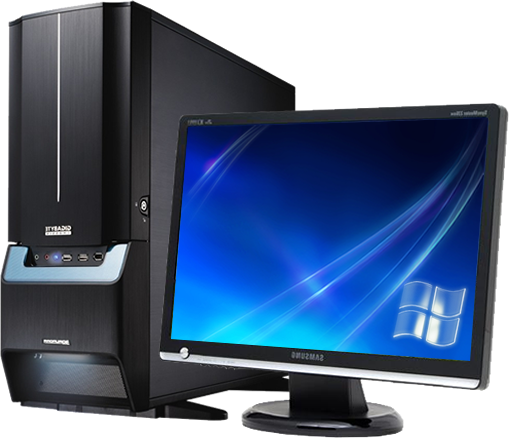
\includegraphics[width=2.5cm]{images/DesktopComputer.png}\\
				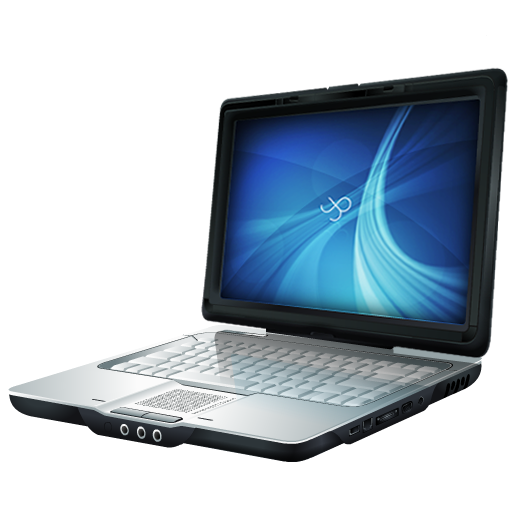
\includegraphics[width=2.3cm]{images/Laptop.png}\\
				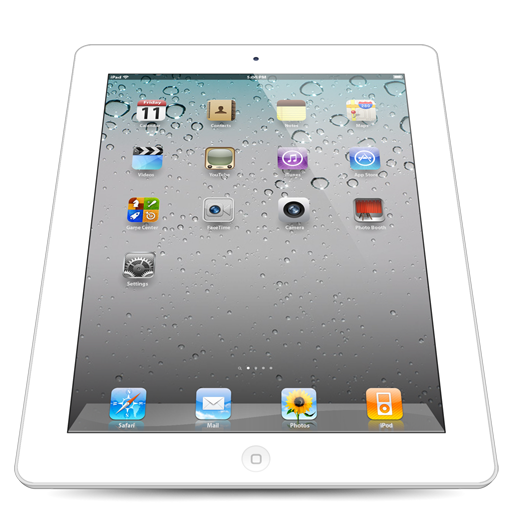
\includegraphics[width=1.5cm]{images/ipad-2-white-perspective.png}\\
			}
			\only<2>{
				{\huge\color{yellow}H}~{\large 人}~{\tiny 感官、情绪、思考}
				\begin{itemize}
					\item 多种感觉
					\item 模式识别
					\item 归纳推理
					\item 多重决策
					\item 适应性、容错
					\item 模糊逻辑
				\end{itemize}
			}
			\only<4>{{\huge\color{yellow}H}~{\large 人}\\灵活、复杂的创造性劳动}
		\end{center}
		\column{5cm}
		\begin{center}
			\only<1,2>{
				
\includegraphics[width=1.5cm]{images/07.png}
				
\includegraphics[width=1.5cm]{images/10.png}\\
				
\includegraphics[width=1.5cm]{images/04.png}
				
\includegraphics[width=1.5cm]{images/05.png}\\
				
\includegraphics[width=1.5cm]{images/13.png}
				
\includegraphics[width=1.5cm]{images/15.png}\\
			}
			\only<3>{
				{\huge\color{blue}C}~{\large 计算机}~{\tiny 设备、结构、算法、数据}
				\begin{itemize}
					\item 精确计数
					\item 准确存取
					\item 快速、一致响应
					\item 数据处理能力
					\item 循环重复
					\item 简单和清晰的任务
				\end{itemize}
			}
			\only<4>{{\huge\color{blue}C}~{\large 计算机}\\清晰、重复的大规模任务}
		\end{center}
	\end{columns}
\end{frame}

\begin{frame}
	\frametitle{什么是人机交互~\color{yellow}{H}\color{cyan}{C}\color{green}{I}}
	\beamertemplatetransparentcovereddynamicmedium
	\onslide<1->{{\huge\color{green}I}~交互的宗旨:}
	\onslide<2->{让人机各展所长}
	\begin{itemize}
		\item<3-> {\small The study of people and computing and the way they influence each other}
		\item<4-> {\small A set of processes, dialogues, and actions through which a human user employs and interacts with a computer}
		\item<5-> {\small A discipline concerned with the design, evaluation and implementation of interactive computing systems for human use with the study of major phenomena surrounding them.}
		\item<6-> 人机交互是关于\textbf{设计}、\textbf{评价}和\textbf{实现}供人们使用的交互式计算机系统,且围绕这些方面的主要现象进行研究的科学\\
			{\tiny\textit{ACM SIGCHI, 1992, Curricula for Human-Computer Interaction}}
	\end{itemize}
\end{frame}

\begin{frame}
	\frametitle{什么是人机交互~\color{yellow}{H}\color{cyan}{C}\color{green}{I}}
	\begin{columns}
		\column{5cm}
		\begin{itemize}
			\item {\large 人}\\~~{\tiny 计算机程序最终用户}
			\item {\large 计算机}\\~~{\tiny 程序的载体}
			\item {\large 交互}
			\begin{itemize}
				\item {\tiny 人告诉计算机应该做什么}
				\item {\tiny 计算机反馈任务结果}
			\end{itemize}
		\end{itemize}
		\column{5cm}
		\begin{tikzpicture}[node distance=1cm, auto,]
			\node[] (dummy) {};
			\node[punkt, above=of dummy]	(human)	{Human};
			\node[punkt, below=of dummy]	(computer)	{Computer};
			\node[left=of dummy]	(input)	{Input};
			\node[right=of dummy]	(output)	{Output};
			\path[line]	(human)--(input);
			\path[line]	(input)--(computer);
			\path[line]	(output)--(human);
			\path[line]	(computer)--(output);
		\end{tikzpicture}
	\end{columns}
\end{frame}

\begin{frame}
	\frametitle{人机交互的目的}
	\beamertemplatetransparentcovereddynamicmedium
	\transwipe
	\begin{itemize}[<+->]
		\item 提高生产力、降低成本:
		\begin{itemize}
			\item 安全:
			\begin{itemize}
				\item 系统是否够强壮可靠?
				\item 例如这些场景:核电站运转,航空管理
			\end{itemize}
			\item 功能:
			\begin{itemize}
				\item 系统支持多丰富的任务?
			\end{itemize}
			\item 效率:
			\begin{itemize}
				\item 完成任务需要消耗多少资源?
			\end{itemize}
			\item 易用性:
			\begin{itemize}
				\item 学习使用这套系统需要多少时间精力?
			\end{itemize}
		\end{itemize}
		\item 然而\dots
		\begin{itemize}
			\item 更丰富、全面的功能是以易用性为代价的
			\item 也更易让用户混淆
		\end{itemize}
	\end{itemize}
\end{frame}

\begin{frame}
	\frametitle{人机交互的目的}
	\beamertemplatetransparentcovereddynamicmedium
	\transwipe
	\setbeamercolor{uppercol}{fg=white,bg=green!80!gray}
	\setbeamercolor{lowercol}{fg=black,bg=green!20!white}
	\onslide<1->{
		\begin{beamerboxesrounded}[upper=uppercol,lower=lowercol,shadow=true]{当前}
			\begin{itemize}
				\item 计算机已经影响到几乎社会的每一处角落
				\item 一个小的变化将影响到很大的层面
				\item 数一数自己身边有多少计算机
			\end{itemize}
		\end{beamerboxesrounded}
	}
	\onslide<2->{
		\begin{beamerboxesrounded}[upper=uppercol,lower=lowercol,shadow=true]{因而}
			在如此大的规模之下,人群没有那么容易去适应系统,系统设计应该贴近人们的需求来进行。
		\end{beamerboxesrounded}
	}
\end{frame}

\begin{frame}
	\frametitle{人机交互五要素}
	\begin{itemize}
		\item 目标~{\small 用户需求的直接反映}
		\item 可视性~{\small 将控制功能及信息良好的展现出来}
		\item 反馈~{\small 及时准确的将状态告知用户}
		\item 可供性~{\small 容易被察觉和接受的功能设计}
		\item 任务~{\small 所需执行的具体操作}
	\end{itemize}
\end{frame}

\begin{frame}
	\frametitle{涉及到的相关学科}
	\begin{itemize}
		\item Cognitive psychology 认知心理学
		\item Ergonomics 人体工程学
		\item Linguistics 语言学
		\item Artificial intelligence 人工智能
		\item Sociology and social psychology 社会学及社会心理学
		\item Engineering and industrial design 工程及工业设计
	\end{itemize}
\end{frame}

\subsection{主要研究内容}
\begin{frame}
	\frametitle{主要研究内容}

\end{frame}

\subsection{发展史}
\begin{frame}
	\frametitle{发展史}

\end{frame}

\begin{frame}
	\frametitle{鼠标的故事}

\end{frame}

\begin{frame}
	\frametitle{语音的故事}

\end{frame}

\begin{frame}
	\frametitle{体感的故事}

\end{frame}

\subsection{应用}
\begin{frame}
	\frametitle{应用}

\end{frame}

\section{小节}
\begin{frame}
	\frametitle{小节}
	\begin{itemize}
		\item 了解人机交互技术
		\begin{itemize}
			\item {\small 基本概念、研究内容、发展趋势、典型应用}
		\end{itemize}
		\item 探讨课程价值~{\tiny 拓展兴趣方向,对今后的学习、研究、工作带来不一样的想法}
	\end{itemize}
\end{frame}

\end{document}